\chapter{Analysis}

Measurement results / analysis / discussion: 1/3

\begin{itemize}
\item whatever you have done, you must comment it, compare it to other systems, evaluate it
\item usually, adequate graphs help to show the benefits of your approach
\item caution: each result/graph must be discussed! what's the reason for this peak or why have you ovserved this effect
\end{itemize}

\section{Transmitted image size}
\begin{figure}[H]
\centering
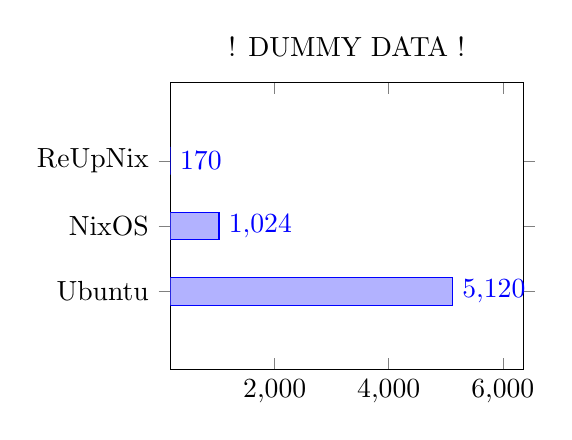
\begin{tikzpicture}
  \begin{axis}[
    title  = ! DUMMY DATA !,
    xbar,
    ytick             = data,
    enlarge y limits  = 0.6,
    enlarge x limits  = { 0.25, upper},
    width = 0.5\textwidth,
    symbolic y coords = {Ubuntu, NixOS, ReUpNix},
    nodes near coords,
  ]
  \addplot coordinates { (170,ReUpNix)         (1024,NixOS)
                         (5120,Ubuntu)   };
  \end{axis}
\end{tikzpicture}
\caption{Image size by OS in megabytes}
\end{figure}

\section{Disk usage}
\begin{figure}[H]
\centering
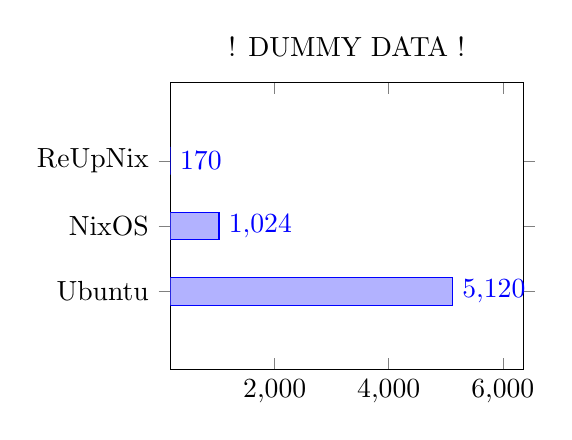
\begin{tikzpicture}
  \begin{axis}[
    title  = ! DUMMY DATA !,
    xbar,
    ytick             = data,
    enlarge y limits  = 0.6,
    enlarge x limits  = { 0.25, upper},
    width = 0.5\textwidth,
    symbolic y coords = {Ubuntu, NixOS, ReUpNix},
    nodes near coords,
  ]
  \addplot coordinates { (170,ReUpNix)         (1024,NixOS)
                         (5120,Ubuntu)   };
  \end{axis}
\end{tikzpicture}
\caption{Disk utilization after boot by OS in megabytes}
\end{figure}

\section{Mean time to recover}
\begin{figure}[H]
\centering
\begin{tikzpicture}
  \begin{axis}[
    title  = ReUpNix,
    ybar,
    enlarge y limits  = {0.15,upper},
    width = 0.5\textwidth,
    nodes near coords,
  ]
    \addplot table [x=seconds, y=times, col sep=comma] {data/time-to-recover-reupnix.csv};
  \end{axis}
\end{tikzpicture}
\begin{tikzpicture}
  \begin{axis}[
    title  = NixOS,
    ybar,
    enlarge y limits  = {0.15,upper},
    width = 0.5\textwidth,
    nodes near coords,
  ]
    \addplot table [x=seconds, y=times, col sep=comma] {data/time-to-recover-nixos.csv};
  \end{axis}
\end{tikzpicture}
\begin{tikzpicture}
  \begin{axis}[
    title  = Ubuntu 22.04,
    ybar,
    enlarge y limits  = {0.15,upper},
    width = 0.5\textwidth,
    nodes near coords,
  ]
    \addplot table [x=seconds, y=times, col sep=comma] {data/time-to-recover-ubuntu.csv};
  \end{axis}
\end{tikzpicture}
\caption{Time of recovery after a reboot by OS in seconds.}
\end{figure}
